\newpage
\section{Programming exercise : Implementing Logistic Regression and Neural Networks \problemworth{50}}

\section*{Introduction}

\begin{figure}[ht]
\centering
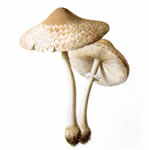
\includegraphics[scale=2.5]{mushroom.jpg}
\end{figure}

In this problem, we will continue to work on the mushroom classification task which was used in HW1. The dataset is adapted from the \href{https://archive.ics.uci.edu/ml/datasets/mushroom}{UCI Machine Learning Repository} and it contains descriptions of hypothetical samples corresponding to 23 species of gilled mushrooms. Each mushroom is described in terms of physical characteristics, and the goal is to classify mushrooms as \emph{edible} or \emph{poisonous}. We will apply decision trees and k-nearest neighbors. Since this dataset is relatively simple for classification, we only use 6 features out of 22 features in the original dataset. Features we use include: 
cap-shape, cap-color, gill-color, stalk-root, veil-type, ring-number.

\begin{comment} % Expected to be covered in the discussion session
\section*{Starter Files}
\vspace{-\baselineskip}
\rule{\textwidth}{1pt}
code and data
\begin{itemize}[nolistsep]
\item Code: \href{https://colab.research.google.com/drive/1A4W-Zyf9KJqzQKHMXPgv26Zj-__GDje-?usp=sharing}{Fall2021-CS146-HW1.ipynb}\item Data: \href{https://drive.google.com/drive/folders/1xjZlT1TzoJ79Hd48fdjI1-gk7hnNOwTz?usp=sharing}{nutil.py and adult\_subsample.csv} 
\end{itemize}
documentation
\begin{itemize}[nolistsep]
\item Decision Tree Classifier: \\{\footnotesize \url{http://scikit-learn.org/stable/modules/generated/sklearn.tree.DecisionTreeClassifier.html}}
\item K-Nearest Neighbor Classifier: \\{\footnotesize \url{http://scikit-learn.org/stable/modules/generated/sklearn.neighbors.KNeighborsClassifier.html}} 
\item Cross-Validation: \\{\footnotesize \url{https://scikit-learn.org/stable/modules/generated/sklearn.model_selection.StratifiedShuffleSplit.html}}
\item Metrics: \\ {\footnotesize \url{http://scikit-learn.org/stable/modules/generated/sklearn.metrics.accuracy_score.html}, \\
\url{https://scikit-learn.org/stable/modules/generated/sklearn.metrics.f1_score.html?highlight=f1%20score#sklearn.metrics.f1_score}} 
\item Data Preprocessing: \\{\footnotesize \url{https://scikit-learn.org/stable/modules/generated/sklearn.preprocessing.StandardScaler.html?highlight=standardscaler#sklearn.preprocessing.StandardScaler}}
\end{itemize}
\vspace{-\baselineskip}
\rule{\textwidth}{1pt}

Note that any portions of the code that you must modify have been indicated with \verb|TODO|. Do not change any code outside of these blocks.

\ifsoln
\else
\clearpage
\fi
\end{comment}


For all the coding, please refer to the following Colab notebook
\href{https://colab.research.google.com/drive/1QSVDbmWZHVEye__A1wC9u6qhycnUG1Ks?usp=sharing}{Fall2022-CM146-HW2.ipynb}. 

% \href{https://colab.research.google.com/drive/1GIF6z5lIptFAQYVXQIM4eCfi__yY6txS?usp=sharing}{Fall2022-CM146-HW1.ipynb}. 

\textbf{Before executing or writing down any code, please make a copy of the notebook and save it to your own google drive by clicking the “File” $\rightarrow$ “Save a copy in Drive”.} 

\begin{figure}[ht]
\centering
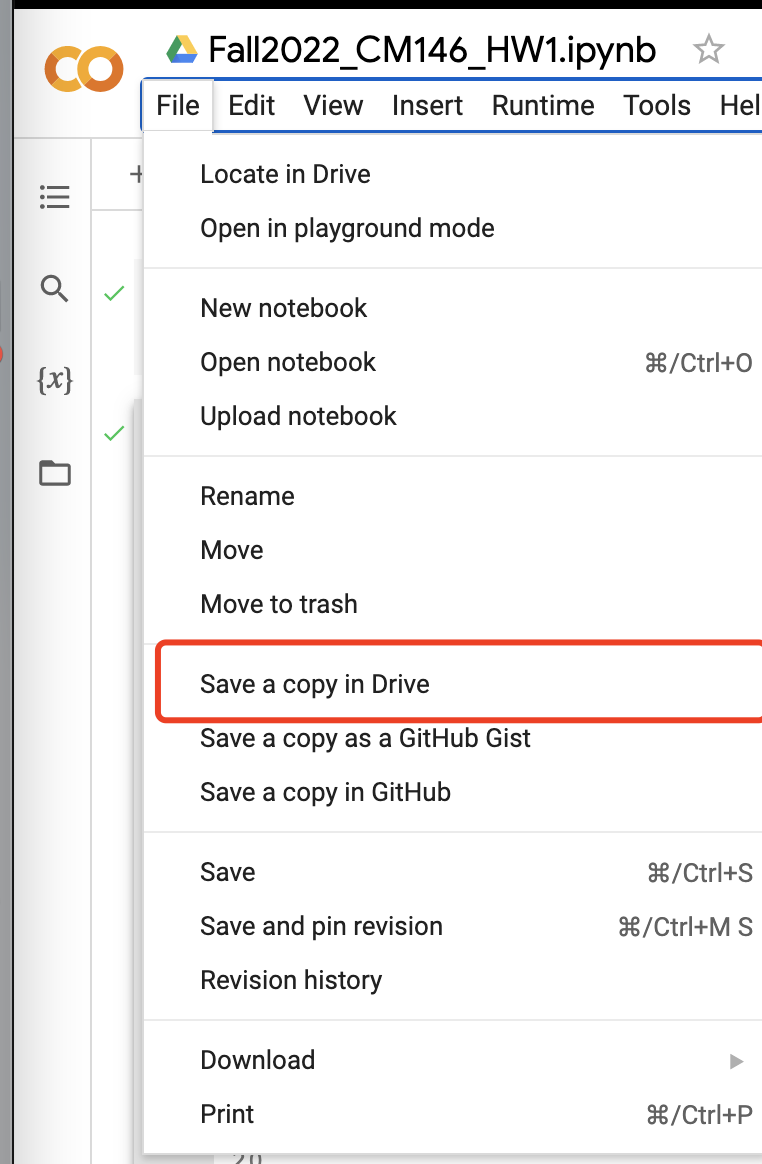
\includegraphics[scale=0.25]{save-colab-to-drive.png}
\end{figure}

You will probably be prompted to log into your Google account. Please make sure all the work you implement is done on your own saved copy. You won’t to able to make changes on the the original notebook shared with the entire class.

The notebook has marked blocks where you need to code:
\begin{verbatim}
### ========== TODO : START ========== ###
### ========== TODO : END ========== ###
\end{verbatim}

\section*{Submission instructions for programming problems}
\begin{itemize}
\item Please save the execution output in your notebook. When submitting, please export the notebook to a \verb|.ipynb| file by clicking ``File'' $\rightarrow$ ``Download .ipynb'' and upload the notebook to BruinLearn.

\item
Your code should be commented appropriately. Importantly:
\begin{itemize}[nosep]
\item Your name should be at the top of the file.
\item Each class and method should have an appropriate doctsring.
\item Include some comments for anything complicated.
\end{itemize}

There are many possible solutions to this assignment, which makes coding style and comments important for graders to conveniently understand the code. 
% You may lose points for poorly commented or poorly organized codes.
\item Please submit all the plots and the rest of the solutions (other than codes) to Gradescope.
\end{itemize}

\subsection{Creating Datasets and DataLoaders \problemworth{5}}

Datasets and Dataloaders are pytorch specific wrappers useful for maintaining and batching data. They help in dynamically loading and keeping track of batches while training/inference of machine learning algorithms. We will wrap our current data into datasets and dataloaders for this part.

\begin{enumerate}

\item \itemworth{5} 
Prepare \verb|train_loader|, \verb|valid_loader|, and \verb|test_loader| by using \verb|TensorDataset| and \verb|DataLoader|. We expect to get a batch of pairs $(\mathbf{x}_n, y_n)$ from the dataloader. Please set the train batch size to 16 and test batch size to 32.

You can refer \url{https://pytorch.org/docs/stable/data.html} for more information about \verb|TensorDataset| and \verb|DataLoader|. 

\end{enumerate}

\subsection{One Layer Neural Network \problemworth{11}}

For one-layer network, we consider a network from input dimension to the output dimension. In other words, we learn a $6 \times 1$ weight matrix $\mathbf{W}$. Given a $\mathbf{x}_n$, we can compute the probability of output as $\mathbf{p}_n = \sigma(\mathbf{W}^\top \mathbf{x}_n)$, where $\sigma(.)$ is the sigmoid function.

We will train our network using the \emph{cross entropy loss}. For recap,
$$
-\sum_{n=0}^{N} \sum_{c=0}^{C}  \mathds{1}(c=y_n) \log (\mathbf{p}_{n, c})
$$
where $N$ is the number of examples, $C$ is the number of classes, and $\mathds{1}$ is the indicator function.

\begin{enumerate}
\setcounter{enumi}{1}

\item \itemworth{5}
Prove the equivalence of the current setup of the one-layer network with a logistic regression model. Mainly, we want to show that the predicted output and the loss terms are equivalent for both the models for a given $(\mathbf{x}_n, y_n)$.

\solution{
    For both logistic regression and the one layer neural network, the output function models probability using the same function: $\sigma(W^Tx_n)$, so the output will be the same. The cross entropy loss also simplifies to the loss function used in logistic regression in one layer ($\sum_n log(p_n)$) which we show below. 

    \begin{gather*}
        -\sum_{n=0}^{N} \sum_{c=0}^{C}  \mathds{1}(c=y_n) \log (\mathbf{p}_{n, c}) \\
        = -\sum_{n=0}^N \mathds{1}(y_n=0)log(p_{n,c=0}) + \mathds{1}(y_n=1)log(p_n{n,c=1}) \text{ (one of these terms is 0)}\\
        = -\sum_{n=0}^Nlog(p_n) \\
    \end{gather*}
    $\hfill \Box$
}

\item \itemworth{3}
Implement the constructor of \verb|OneLayerNetwork| with \verb|torch.nn.Linear| and implement the \verb|forward| function to compute the outputs of the single fully connected layer i.e. $\sigma(\mathbf{W}_1^\top \mathbf{x}_n)$. Notice that we use the sigmoid function here as the activation.

You can refer to \url{https://pytorch.org/docs/stable/generated/torch.nn.Linear.html} for more information about \verb|torch.nn.Linear| and \url{https://pytorch.org/docs/stable/generated/torch.nn.Sigmoid.html} for more information about \verb|torch.nn.Sigmoid|.

\item \itemworth{3}
In this part, we will create an instance of the model, set up the loss criterion and initialize the optimizer as well. Create an instance of \verb|OneLayerNetwork|, set up a criterion with \verb|torch.nn.BCELoss| with the aggregation of loss as the sum (see \verb|reduction| parameter), and set up a stochastic gradient descent (SGD) optimizer with learning rate as a parameter using \verb|torch.optim.SGD| \problemworth{2}

You can refer to \url{https://pytorch.org/docs/stable/optim.html} for more information about \verb|torch.optim.SGD|. Since we have only two classes, we use the Binary Cross Entropy Loss - \verb|torch.nn.BCELoss|. We can refer to \url{https://pytorch.org/docs/stable/generated/torch.nn.BCELoss.html} for more information.

\end{enumerate}

\subsection{Two Layer Neural Network \problemworth{6}}

For one-layer network, we consider a network from input dimension to a hidden dimension and then back to the output dimension.In other words, the first layer will consist of a fully connected layer with $6 \times h$ weight matrix $\mathbf{W}_1$ and a second layer consisting of $h \times 1$ weight matrix $\mathbf{W}_2$ where $h$ is the size of the hidden layer. Given a $\mathbf{x}_n$, we can compute the probability vector $\mathbf{p}_n = \sigma(\mathbf{W}_2^\top \sigma(\mathbf{W}_1^\top \mathbf{x}_n))$, where $\sigma(.)$ is the sigmoid function.

\begin{enumerate}
\setcounter{enumi}{4}

\item \itemworth{4}
Implement the constructor of \verb|TwoLayerNetwork| with \verb|torch.nn.Linear| and implement the \verb|forward| function to compute the outputs i.e. $\sigma(\mathbf{W}_2^\top \sigma(\mathbf{W}_1^\top \mathbf{x}_n))$. Notice that we use the sigmoid function here as the activation for both layers.

\item \itemworth{2}
Create an instance of \verb|TwoLayerNetwork|, set up a criterion with \verb|torch.nn.BCELoss| with the aggregation of loss as the sum (see \verb|reduction| parameter), and set up a stochastic gradient descent (SGD) optimizer with learning rate as a parameter using \verb|torch.optim.SGD| \problemworth{2}

\end{enumerate}

\subsection{Training the Model \problemworth{8}}

Once we have initialized both the models, we will train the models. We will be using mini-batch SGD for training the models i.e. instead of computing gradients and updating weights using all examples, we will compute them for a smaller subset. Mini-batch SGD is fast in computation and helps fast convergence while not being too random in terms of gradient directions. You can read up more about the differences of gradient descent and mini-batch SGD here - \url{https://towardsdatascience.com/batch-mini-batch-stochastic-gradient-descent-7a62ecba642a}.

\begin{enumerate}
\setcounter{enumi}{6}

\item \itemworth{8}
We provide you with a base code for batching using the dataloaders created before. You have to implement the training process. This includes initializing gradients to zeros, forward pass over the model, computing the loss, computing the gradients using backpropagation, and updating model parameters. You can refer to following tutorial to understand what each of these steps do - \url{https://pytorch.org/tutorials/recipes/recipes/zeroing_out_gradients.html}.

If you implement everything correctly, after running the \verb|train| function (later in the colab), you should get results similar to the following (numbers can be different, but they should be non-zero). \problemworth{8}

\begin{minted}{text}
Start training OneLayerNetwork...
| epoch  1 | train loss 0.546384 | train acc 0.732357 | valid loss ...
| epoch  2 | train loss 0.537560 | train acc 0.755881 | valid loss ...
| epoch  3 | train loss 0.533699 | train acc 0.761309 | valid loss ...
...
\end{minted}

\end{enumerate}

\subsection{Putting it all together - Performance Evaluation \problemworth{20}}

Now we will run the main code and call these various functions (we have given the code, you have to run it). You should train both the models using the default hyperparameters i.e.

\begin{minted}{text}
lr = 0.001
num_epochs = 50
hidden_size = 6
activation = 'sigmoid'
\end{minted}

\begin{enumerate}
\setcounter{enumi}{7}

\item \itemworth{6}
Now we will compare the performance of both the models by plotting the loss and the accuracies. Generate a plot depicting how \verb|one_train_loss|, \verb|one_valid_loss|, \verb|two_train_loss|, \verb|two_valid_loss| varies with epochs. Include the plot in the report and describe your findings.

Generate a plot depicting how \verb|one_train_acc|, \verb|one_valid_acc|, \verb|two_train_acc|, \verb|two_valid_acc| varies with epochs. Include the plot in the report and describe your findings.

\solution{

    I found that the two layer neural network performed worse initially, but after several more training epochs passed it began to perform better than the single layer neural network.
    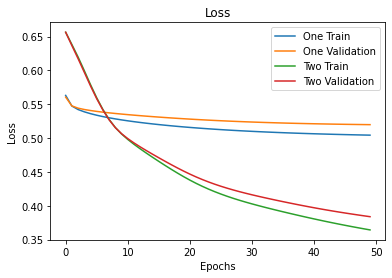
\includegraphics[width=.4\linewidth]{hw2-images/loss-plot.png}
    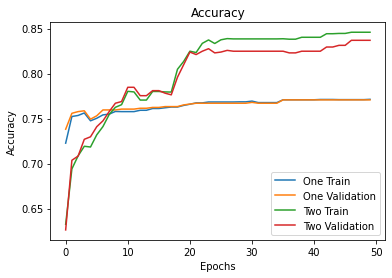
\includegraphics[width=.4\linewidth]{hw2-images/acc-plot.png}
}

\item \itemworth{4}
Calculate and report the test accuracy of both the one-layer network and the two-layer network. Explain why we get such results.

\solution{

    One Layer Accuracy: 0.7798891663551331 and Two Layer Accuracy: 0.8368963003158569. For one layer, the test accuracy is slightly improved from the train accuracy while for two it is slightly lower than train. The differences are quite low so it may just be due to chance and how the data was split between training and test sets. The two layer accuracy is likely higher because it is able to determine a better decision boundary for the data due to the hidden layer.
}

\item \itemworth{5}
Model analysis is a really important component for improving the model performance. In this part, you will implement the function for confusion matrix and create the confusion matrix for the validation data. Report the confusion matrix and your observations for future improvements. You may utilize the \verb|confusion_matrix| library from sklearn - \url{https://scikit-learn.org/stable/modules/generated/sklearn.metrics.confusion_matrix.html}.

\solution{

    One layer NN: $\begin{bmatrix}
        358 & 164 \\
        82 & 469
    \end{bmatrix}$, Two layer NN: $\begin{bmatrix}
        387 & 135 \\
        40 & 511
    \end{bmatrix}$ 

    Observation: In both cases, there are more false positives than false negatives so in the future we could modify our data regularization or training process.
}

\item \itemworth{5}
Neural networks are sensitive to hyperparameters. In this part, you will tune some hyperparameters to improve the model performance further. We will consider only the \verb|TwoLayerNetwork| for the tuning. By changing only the default hyperparameters specified above, show an improvement in the model performance (an improvement of $1$ point in test accuracy will be awarded full credit). Report your old and new model training/validation loss curves, accuracy curves and test accuracies. Also report the new tuned hyperparameter values. 

\solution{

    For hyperparameters:
    \begin{itemize}
        \item lr = 0.002
        \item hidden\_size = 12
        \item activation = `sigmoid'
        \item num\_epochs = 50
    \end{itemize}

    Test accuracy was 0.8733174800872803 up from 0.8368963003158569.

    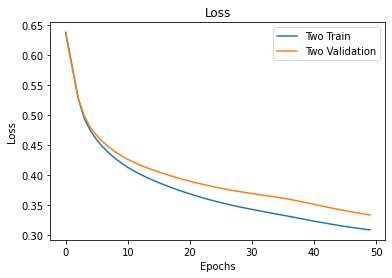
\includegraphics[width=.4\linewidth]{hw2-images/improved-loss-plot.png}
    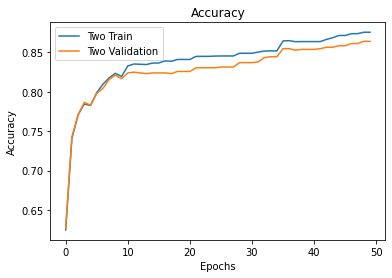
\includegraphics[width=.4\linewidth]{hw2-images/improved-acc-plot.png}
    
    The old curves can be found in part (h).
}
\end{enumerate}